\documentclass{beamer}

\mode<presentation>
{
	\usetheme{CambridgeUS}
	\setbeamercovered{transparent}
}
\usepackage[spanish]{babel}
\usepackage[latin1]{inputenc}
\usepackage{color}
\usepackage{hyperref}
\usepackage{multicol}
\usepackage{algorithm,algorithmic}

\title[\textbf{ICI 4242 - Aut\'omatas y compiladores}]{\textbf{ICI 4242 - Aut\'omatas y compiladores}}

\subtitle{An\'alisis L\'exico}

\author[Rodrigo Olivares]
{
	Rodrigo Olivares \\
	\vspace{0.5mm}
	Mg. en Ingenier\'ia Inform\'atica \\
	\vspace{0.5mm}
	\texttt{\normalsize rodrigo.olivares@uv.cl}
}

\institute[PUCV]

\date{1er Semestre} 

\subject{An\'alisis L\'exico}

%\AtBeginSection
%{
%	\begin{frame}<beamer>
%	\frametitle{Contenido}
%	\tableofcontents[currentsection,currentsubsection]
%	\end{frame}
%}
%
%\AtBeginSubsection
%{
%	\begin{frame}<beamer>
%	\frametitle{Contenido}
%	\tableofcontents[currentsection,currentsubsection]
%	\end{frame}
%}
%
%\beamerdefaultoverlayspecification{<+->}

\begin{document}

	\begin{frame}
		\titlepage
	\end{frame}

%	\begin{frame}
%		\frametitle{Contenido}
%		\tableofcontents[pausesections]
%	\end{frame}

	\section{Funciones del analizador l\'exico}

		%\subsection{Definici\'on}

		\begin{frame}
			\frametitle{Funciones del analizador l\'exico}
			%\framesubtitle{Definici\'on}

			\begin{block}{Definici\'on}
			    \textbf{Analizador l\'exico}: \emph{Corresponde a la primera fase de un compilador}. Es la encargada de recibir el programa fuente, reconocer caracter a caracter cada componente y luego agruparlos, para formar unidades con significado propio, los \emph{componentes l\'exicos} (\textbf{tokens}).
			\end{block}
		\end{frame}

		\begin{frame}
			\frametitle{Funciones del analizador l\'exico}
			%\framesubtitle{Definici\'on}

			\begin{figure}[H]
			    \begin{center}
			        \fbox{\fbox { 
			            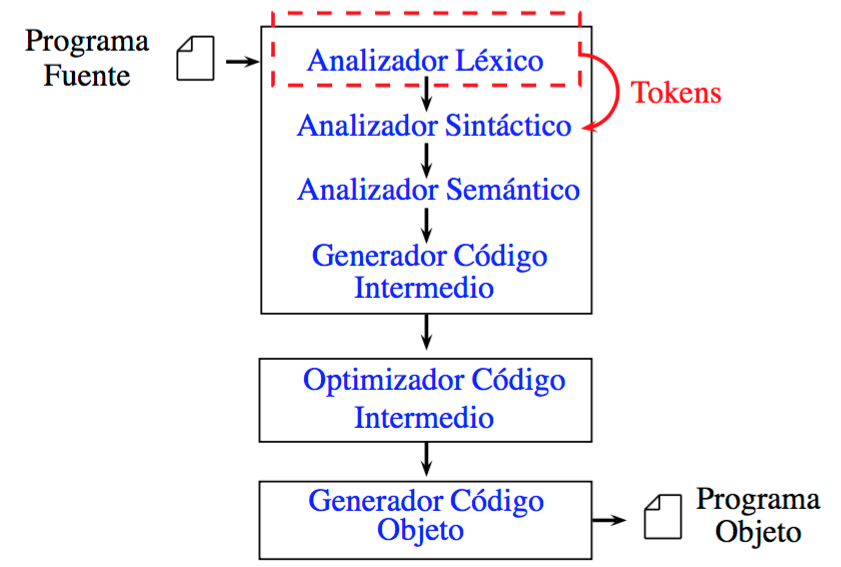
\includegraphics[scale=.3]{images/lex1.png}
			        }}
			    \end{center}
			\end{figure}
		\end{frame}

		\begin{frame}
			\frametitle{Funciones del analizador l\'exico}
			%\framesubtitle{Definici\'on}

			\begin{block}{Estos componentes l\'exicos representan:}
			  \begin{itemize}
			      \item[$\rightarrow$] Palabras reservadas: \textbf{if}, \textbf{while}, \textbf{do}, $\ldots$
			      \item[$\rightarrow$] Identificadores: asociados a variables, nombres de funciones, tipos de datos definidos por el usuario, etiquetas, $\ldots$ Por ejemplo: \textbf{posicion}, \textbf{velocidad}, \textbf{tiempo}, $\ldots$
			      \item[$\rightarrow$] Operadores: $=~*~+~-~/~==~>~<~\&~!=\ldots$
			      \item[$\rightarrow$] S\'imbolos especiales: $;~(~)~[~]~{~}\#\ldots$
			      \item[$\rightarrow$] Constantes num\'ericas: literales que representan valores enteros, punto flotante, etc. Por ejemplo: $982;~0xF678;-83.2E^{+2},\ldots$
			      \item[$\rightarrow$] Constantes de caracteres: literales que representan cadenas concretas de caracteres. Por ejemplo: \textbf{``hola mundo"},$\ldots$
			  \end{itemize}
			\end{block}
		\end{frame}
		
		\begin{frame}
			\frametitle{Funciones del analizador l\'exico}
			%\framesubtitle{Definici\'on}

            \begin{block}{}
                El analizador l\'exico opera bajo petici\'on del analizador sint\'actico, devolviendo un componente l\'exico conforme el analizador sint\'actico lo va necesitando para avanzar en la gram\'atica.
            \end{block}
			\begin{block}{}
                Los componentes l\'exicos son los s\'imbolos terminales de la gram\'atica. Suele implementarse como una subrutina del analizador sint\'actico. 
            \end{block}
            \begin{block}{}
                Cuando recibe la orden \textbf{obt\'en el siguiente componente l\'exico}, el analizador l\'exico lee los caracteres de entrada hasta identificar el siguiente componente l\'exico.
            \end{block}
		\end{frame}		
		
		\begin{frame}
			\frametitle{Funciones del analizador l\'exico}
			%\framesubtitle{Definici\'on}

			\begin{figure}[H]
			    \begin{center}
			        \fbox{\fbox { 
			            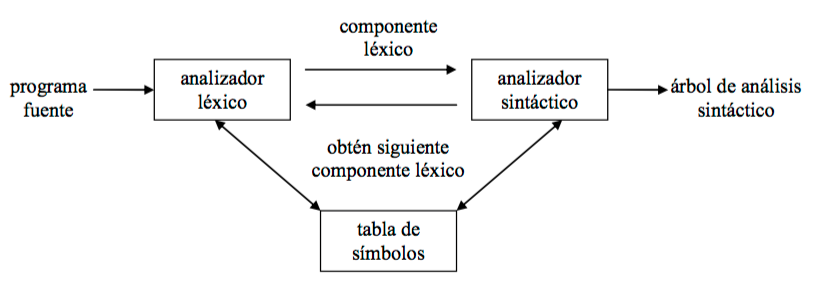
\includegraphics[scale=.35]{images/lex2.png}
			        }}
			    \end{center}
			\end{figure}
		\end{frame}	
		
		\begin{frame}
			\frametitle{Funciones del analizador l\'exico}
			%\framesubtitle{Definici\'on}

			\begin{block}{Otras funciones secundarias:}
			  \begin{itemize}
			      \item[$\rightarrow$] Manejo del archivo de entrada del programa fuente: abrirlo, leer sus caracteres, cerrarlo y gestionar posibles errores de lectura.
			      \item[$\rightarrow$] Eliminar comentarios, espacios en blanco, tabuladores y saltos de l\'inea (caracteres no v\'alidos para formar un \textbf{token}).
			      \item[$\rightarrow$] Inclusi\'on de ficheros: \emph{\#include}, \emph{import}, \emph{required}, etc
			      \item[$\rightarrow$] Contabilizar el n\'umero de l\'ineas y columnas para emitir mensajes de error.
			      \item[$\rightarrow$] Reconocimiento y ejecuci\'on de las directivas de compilaci\'on (por ejemplo, para depurar u optimizar el c\'odigo fuente).
			  \end{itemize}
			\end{block}
		\end{frame}		
		
		\begin{frame}
			\frametitle{Funciones del analizador l\'exico}
			%\framesubtitle{Definici\'on}

			\begin{alertblock}{Patr\'on:}
			    Es una regla que genera la secuencia de caracteres que puede representar a un determinado componente l\'exico (una expresi\'on regular).
			\end{alertblock}
			\begin{alertblock}{Lexema:}
			    Cadena de caracteres que concuerda con un patr\'on que describe un componente l\'exico. Un componente l\'exico puede tener uno o infinitos lexemas. Por ejemplo: palabras reservadas tienen un \'unico lexema. Los n\'umeros y los identificadores tienen infinitos lexemas.
			\end{alertblock}
		\end{frame}		
		
		\begin{frame}
			\frametitle{Funciones del analizador l\'exico}
			%\framesubtitle{Definici\'on}

            \begin{table}
                \begin{center}
			         \begin{tabular}{|l|l|l|} \hline
			         \textbf{Componente l\'exico} & \textbf{Lexema} & \textbf{Patr\'on} \\ \hline \hline
			         \textbf{identificador} & indice, a, temp & letra seguida de letras o d\'igitos \\
			         \textbf{num\_entero} & 1492, 1, 2 & d\'igito seguido de m\'as d\'igitos \\
			         \textbf{if} & if & letra i seguida de letra f \\
                    \textbf{do} & do & letra d seguida de o \\
                    \textbf{op\_div} & / & caracter / \\
                    \textbf{op\_asig} & = & caracter = \\ \hline
			        \end{tabular}
			    \end{center}
			\end{table}
		\end{frame}				

		\begin{frame}
			\frametitle{Funciones del analizador l\'exico}
			%\framesubtitle{Definici\'on}

			\begin{alertblock}{}
			    Los componentes l\'exicos se suelen definir como un tipo enumerado. Se codifican como enteros. Tambi\'en se suele almacenar la cadena de caracteres que se acaba de reconocer (el lexema), que se usar\'a posteriomenete para el an\'alisis sem\'antico. \\
			    \vspace{.5cm}
			        \hspace{3cm} \texttt{typedef enum \{ \\
			        \hspace{4cm} TKN\_IF, \\
			        \hspace{4cm} TKN\_THEN, \\
			        \hspace{4cm} TKN\_NUM, \\
			        \hspace{4cm} TKN\_ID, \\
			        \hspace{4cm} TKN\_OPADD,\\
			        \hspace{4cm} $\vdots$ \\
			        \hspace{3cm} \} TokenType;}
			\end{alertblock}
		\end{frame}		

		\begin{frame}
			\frametitle{Funciones del analizador l\'exico}
			%\framesubtitle{Definici\'on}

			\begin{alertblock}{}
			    Es importante conocer el lexema (para construir la tabla de s\'imbolos). Los componentes l\'exicos se representan mediante una estructura registro con tipo de token y lexema: \\
			    \vspace{.5cm}
			        \hspace{1cm} \texttt{typedef struct \{ \\
			        \hspace{1.9cm} TokenType token; \\
			        \hspace{1.9cm} char $^*$lexema; // se reserva memoria din\'amicamente \\
			        \hspace{1cm} \} TokenRecord; \\
			        \hspace{1cm} TokenRecord getToken(void);}
			\end{alertblock}
		\end{frame}	

		\begin{frame}
			\frametitle{Funciones del analizador l\'exico}
			%\framesubtitle{Definici\'on}

			\begin{exampleblock}{Ejemplo}
			    $a[indice] = 2 + 4$ \\
			    \hspace{.5cm}
			    \begin{table}[H]
			        \begin{center}
			            \begin{tabular}{|c|c|c|c|c|c|c|c|c|c|c|c|c|c|c|c|c|c|c|c|} 
			                \multicolumn{20}{l}{buffer de entrada} \\  \hline
			                & a & [ & i & n & d & i & c & e & ] & & = & & 2 & + & 4 & & & & \\ \hline
			                \multicolumn{1}{c}{$\uparrow$} & \multicolumn{19}{l}{} \\  
			            \end{tabular}
			        \end{center}
			    \end{table}
			\end{exampleblock}
		\end{frame}		

		\begin{frame}
			\frametitle{Funciones del analizador l\'exico}
			%\framesubtitle{Definici\'on}

			\begin{exampleblock}{Ejemplo: Cada componente l\'exico va acompa\~nado de su lexema:}
			    \hspace{1cm} \texttt{$<$TKN\_ID, a$>$} \\
			    \hspace{1cm} \texttt{$<$TKN\_CORC\_APER, $[>$} \\
			    \hspace{1cm} \texttt{$<$TKN\_ID, indice$>$} \\
			    \hspace{1cm} \texttt{$<$TKN\_CORC\_CIER, $]>$} \\
			    \hspace{1cm} \texttt{$<$TKN\_NUM, 2$>$} \\
			    \hspace{1cm} \texttt{$<$TKN\_OP\_ADD, $+>$} \\ 
			    \hspace{1cm} \texttt{$<$TKN\_NUM, $4>$}
			\end{exampleblock}
		\end{frame}		

	\section{Especificaci\'on de los componentes l\'exicos}
	
	    \subsection{Expresiones regulares}

		\begin{frame}
			\frametitle{Especificaci\'on de los componentes l\'exicos.}
			\framesubtitle{Expresiones regulares}

			\begin{exampleblock}{}
			    Los componentes l\'exicos se especifican haciendo uso de expresiones regulares. Adem\'as de las tres operaciones b\'asicas: \textbf{concatenaci\'on}, \textbf{repetici\'on} ($^*$) y \textbf{alternativas/uni\'on} ($|$), se usar\'an los siguientes metas\'imbolos:
			    \begin{itemize}
			        \item[$\rightarrow$] \textbf{Una o m\'as repeticiones} $+$
			        \begin{itemize}
			            \item[$\rightarrow$] $\alpha^{+}$ indica una o m\'as repeticiones de $\alpha$
			            \item[$\rightarrow$] $(0|1)^{+} = (0|1)(0|1)^{*}$ $\Leftrightarrow$ $\alpha^{+} = \alpha.\alpha^{*}$
			        \end{itemize}
                    \item[$\rightarrow$] \textbf{Cualquier caracter .}
                    \begin{itemize}
			            \item[$\rightarrow$] $.^{*}b.^{*}$ indica cualquier cadena que contiene una letra b
                    \end{itemize}
                    \item[$\rightarrow$] \textbf{Cualquier car\'acter excepto un conjunto dado \textasciitilde}
                    \begin{itemize}
                        \item[$\rightarrow$] \textasciitilde(a$|$b) indica cualquier caracter que no sea una a \'o b
                    \end{itemize}
                    \item[$\rightarrow$] \textbf{Opcionalidad ?}
                    \begin{itemize}
                        \item[$\rightarrow$] $\alpha$? indica que la expresi\'on $\alpha$ puede aparecer o no. En el caso de que aparezca, s\'olo lo har\'a una vez.
                    \end{itemize}
			    \end{itemize}
			\end{exampleblock}
		\end{frame}		

		\begin{frame}
			\frametitle{Especificaci\'on de los componentes l\'exicos.}
			\framesubtitle{Expresiones regulares}

			\begin{exampleblock}{}
			    Los componentes l\'exicos se especifican haciendo uso de expresiones regulares. Adem\'as de las tres operaciones b\'asicas: \textbf{concatenaci\'on}, \textbf{repetici\'on} ($^*$) y \textbf{alternativas/uni\'on} ($|$), se usar\'an los siguientes metas\'imbolos:
			    \begin{itemize}
			        \item[$\rightarrow$] \textbf{Un rango de caracteres} [ ] (\textbf{clase})
			        \begin{itemize}
			            \item[$\rightarrow$] [a-z] indica cualquier caracter entre la a y z \textbf{min\'usculas}.
			            \item[$\rightarrow$] [a-zA-Z] indica cualquier letra del abecedario min\'uscula o may\'uscula.
			            \item[$\rightarrow$] [0-9] indica cualquier d\'igito de 0 a 9.
			            \item[$\rightarrow$] [abc] indica \emph{a}$|$\emph{b}$|$\emph{c}.
			        \end{itemize}
			    \end{itemize}
			\end{exampleblock}
			\begin{alertblock}{Uso}
			   Cuando queremos usar estos s\'imbolos con su significado tenemos que usar la barra de escape, [a$\backslash$-z] significar\'ia cualquier letra que sea \textbf{a}, \textbf{gui\'on} \'o \textbf{z}.
			\end{alertblock}
		\end{frame}		

		\begin{frame}
			\frametitle{Especificaci\'on de los componentes l\'exicos.}
			\framesubtitle{Expresiones regulares}

            \begin{exampleblock}{Ejemplos}
			   \begin{itemize}
			       \item[$\rightarrow$] N\'umeros
			       \begin{itemize}
			           \item[$\rightarrow$] nat = $[0-9]^{+}$
			           \item[$\rightarrow$] signedNat = $( + | - )$? nat
			           \item[$\rightarrow$] number = signedNat(``."nat)? (E signedNat)?
			       \end{itemize}
			       \item[$\rightarrow$] Identificadores
			       \begin{itemize}
			           \item[$\rightarrow$] letter = [a-zA-Z]
			           \item[$\rightarrow$] digit = [0-9]
			           \item[$\rightarrow$] identifier = letter (letter $|$ digit)$^*$
			       \end{itemize}
			       \item[] Palabras Reservadas
			       \begin{itemize}
			           \item[$\rightarrow$] TKN\_IF = ``if"
			           \item[$\rightarrow$] TKN\_WHILE = ``while"
			           \item[$\rightarrow$] TKN\_DO = ``do"			       
			       \end{itemize}
			   \end{itemize}
			\end{exampleblock}
		\end{frame}		

		\begin{frame}
			\frametitle{Especificaci\'on de los componentes l\'exicos.}
			\framesubtitle{Aut\'omata Finito Determinista}
			
			\begin{figure}[H]
			    \begin{center}
			        \fbox{\fbox { 
			            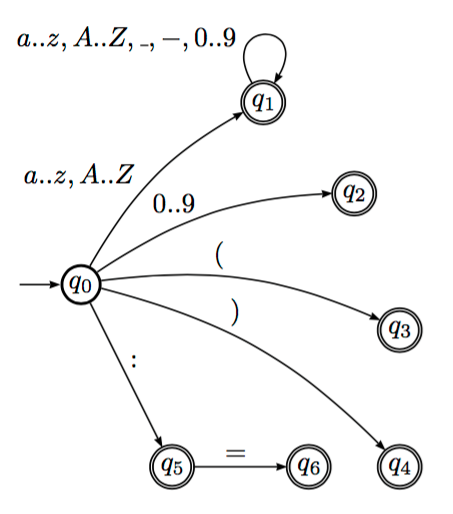
\includegraphics[scale=.35]{images/afd.png}
			        }}
			    \end{center}
			\end{figure}
		\end{frame}	

		\begin{frame}
			\frametitle{Preguntas}

			\hspace{4cm}\huge{Preguntas ?}
		
		\end{frame}
	\end{document}

\usetheme{default}
\usetheme{JuanLesPins}
\usetheme{Goettingen}
\usetheme{Szeged}
\usetheme{Warsaw}

\usecolortheme{crane}

\usefonttheme{serif}
\usefonttheme{structuresmallcapsserif}
 